\documentclass[solutions.tex]{subfiles}

\xtitle

\begin{document}
\maketitle
\begin{exercise}[p. $8$] $[\ldots]$ As an exercise you can redraw them for
negative $v$.
\end{exercise}

This is an "optional" exercise from section $1.2$: we're considering
two reference frames, one static (ours) and one moving at velocity $v$,
in a one-spatial dimension setting. In the graph below:
\begin{itemize}
	\item $x_s(t)$ ($s$ for static) represents the coordinates over
	time of our fixed reference frame;
	\item $x_m(t)$ ($m$ for moving) represents the coordinates over
	time of the moving reference frame; we're assuming the velocity
	to be oriented negatively (i.e. $v < 0$)
	\item $x^\pm_l(t)$ ($l$ for light) represents the coordinates over
	time of a light ray being emited to the left/right, in the (unique)
	spatial direction.
\end{itemize}

Where all those position functions are given in the \textit{static
frame of reference}.

\begin{figure}[H]
	\centering
	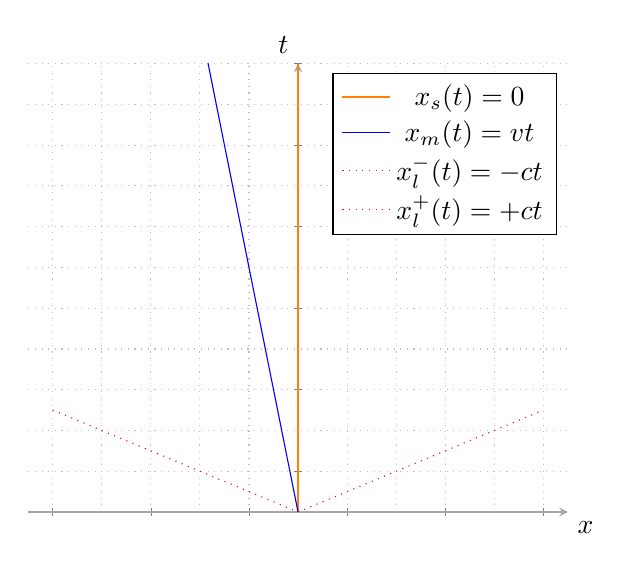
\begin{tikzpicture}[scale=1]
		\begin{axis}[
			xmin=-5.5, xmax=5.5,
			ymin=0, ymax=5.5,
			axis lines=center,
			axis lines=middle,
			axis line style={gray!70},
			ticks=none,
			minor tick num=1,
			xlabel={$x$}, xlabel style={below right},
			ylabel={$t$}, ylabel style={above left},
			minor grid style={dotted},
			major grid style={dotted},
			grid=both,
		]
		\addplot [samples=2, orange, thick] coordinates {(0,0)(0,5.5)};
		\addlegendentry{$x_s(t) = 0$};
		\addplot [samples=2, blue] {-3*x};
		\addlegendentry{$x_m(t) = vt$};
		\addplot [samples=2, red, dotted] {-0.25*x};
		\addlegendentry{$x^-_l(t) = -ct$};
		\addplot [samples=2, red, dotted] {+0.25*x};
		\addlegendentry{$x^+_l(t) = +ct$};
		\end{axis}
	\end{tikzpicture}
\end{figure}
\begin{remark} Note that this is just the mirror image of
what we would have with positive velolicities (reflection
about the vertical $t$ axis).
\end{remark}
\begin{remark} I'll do my best to use an unambiguous notation.
The authors for instance in their graphic $1.$ use the same symbol
"$x$" to denote three distinct things:
\begin{itemize}
	\item Two position functions ($x^+_l(t)$ and $x_m(t)$)
	\item The spatial coordinate of an arbitrary, punctual event.
\end{itemize}
\end{remark}
\begin{exercise}[p. $10$] $[\ldots]$ Can we invert the relationship? That's
easy and I will leave it to you.
\end{exercise}
This is a second optional exercise, a little bit later in the same $1.2$
section, in the same setting of two frames, one static, one moving at
a constant velocity (speed of $v$). \\

Suppose an event $(x_0, t_0)_s$ happens, where I've used the $s$ subscript
to indicate that the coordinates are to be understood within the \textit{static}
frame of reference. The authors just showed us how we could express
the coordinates of this event in the moving reference frame, say
$(x_0', t_0')_m$, where the $m$ subscript indicates that the coordinates
are expressed in the \textit{moving} reference frame. \\

And we're asked to do the thing in the reverse order. So, assume we're
given an event of coordinate $(x_0', t_0')_m$ in the moving frame. We're
looking to express its coordinates $(x_0, t_0)_s$ in the static frame
in terms of $(x_0', t_0')_m$:
\[
	x_0 = f(x_0', t_0');\qquad t_0 = g(x_0', t_0')
\]
By assumption, time flows equally in all reference frames\footnote{In
\textit{this} very peculiar context}, hence:
\[
	\boxed{t_0 = t_0'}
\]

Now if an event happens at position $x_0'$ at a given time ($t_0'=t_0$)
in the moving frame of reference, to express it in the static frame of
reference, we need to take into account the relative motion between
the two frames. As one of them is static, this relative motion is solely
equivalent to the motion of the moving frame. Furthermore,
there's only one spatial dimension, so we just need to shift the position
by how much the moving frame has moved at the given time $t_0'=t_0$:
\[
	x_0 = x_0'+x_m(t_0')\qquad\Leftrightarrow\qquad
	\boxed{x_0 = x_0'+vt_0'}
\]
How do we know this should be a $+$ and not a $-$ thought? Well, because
this is a very simple case, we can take some shortcuts, but it might
help to consider things a bit more generally: the moving frame moves
at some velocity $\bm{v}$, whose spatial coordinates expressed in the
static frame are:
\[
	\bm{v} = \begin{pmatrix}
		v \\
		0 \\
		0 \\
	\end{pmatrix}_s\qquad\text{with } v > 0
\]
Note however that from the point of view of the moving reference frame,
the static frame "moves" with a velocity $\bm{v}'$:
\[
	\bm{v}' = \begin{pmatrix}
		-v \\
		0 \\
		0 \\
	\end{pmatrix}_m\qquad\text{still with } v > 0
\]
This speed now has a \textit{negative} velocitity in the $x$-axis, because
the "static" frame is apparently "moving" away to the left of the "moving"
frame. \\

That's to say, the previous $+$ sign is "arbitrary" somehow, it's just a way
to take into account the effect of this relative motion. \\

One more thought: this is true for any event, so we could use $x$ and
$t$ instead of $x_0$ and $t_0$ to signify that it's true on the full space
instead of at a peculiar point. It's true in particular for all points
describing the motion of the ray of light $x^+_l(t)$:
\[
	ct =: x^+_l(t) = x' + vt\qquad\Leftrightarrow\qquad
		x' = (c-v)t = (c-v)t'
\]

% TODO: reread, perhaps use some matrix/vector transformation to
% clarify some of the confusing t / t'
\end{document}
